\subsection{Implémentation}
\label{res_filtre_num}
Afin de s'assurer de l'implémentation correcte du filtre numérique, celui-ci a été réalisé en 3 étapes :
\begin{enumerate}
\item En Python avec virgule flottante.
\item En Python avec virgule fixe.
\item En C en virgule fixe pour une implémentation directe dans le dsPic.
\end{enumerate}

La première étape nous a servi d'exemple de sorties à avoir dans notre implémentation réelle. Pour ce faire, une sinusoïde a été générée aux fréquences centrales de 900 Hz et 1100 Hz ainsi qu'à 1000 Hz dans le but d'assurer que le signal de la sinusoïde est correctement filtrée.
\begin{figure}[H]
    \centering
    % Première image
    \begin{subfigure}[b]{0.75\textwidth}
        \centering
        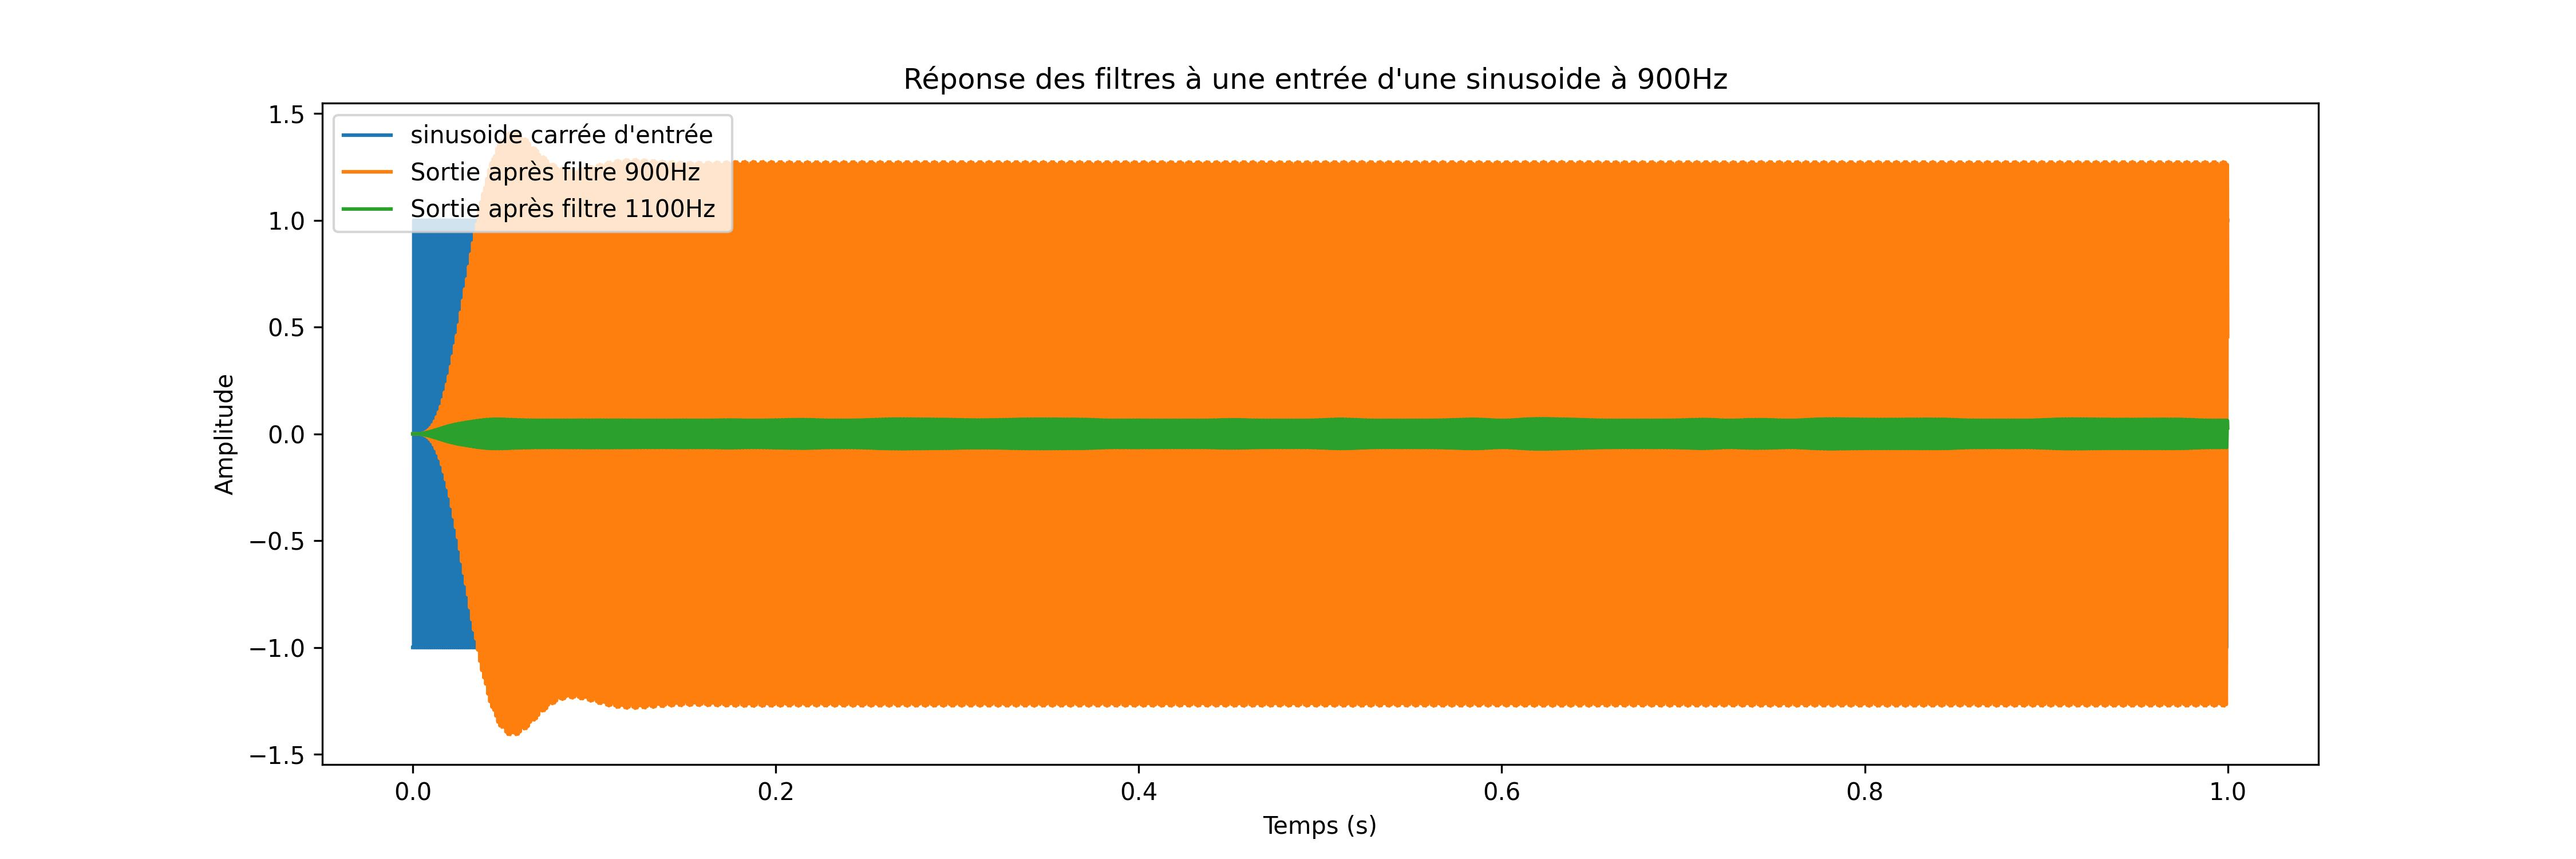
\includegraphics[width=\textwidth]{Pictures/graphique_900Hz.jpeg}
        \caption{Sortie de la sinusoide à 900Hz}
        \label{fig:image1}
    \end{subfigure}
    % Deuxième image
    \begin{subfigure}[b]{0.75\textwidth}
        \centering
        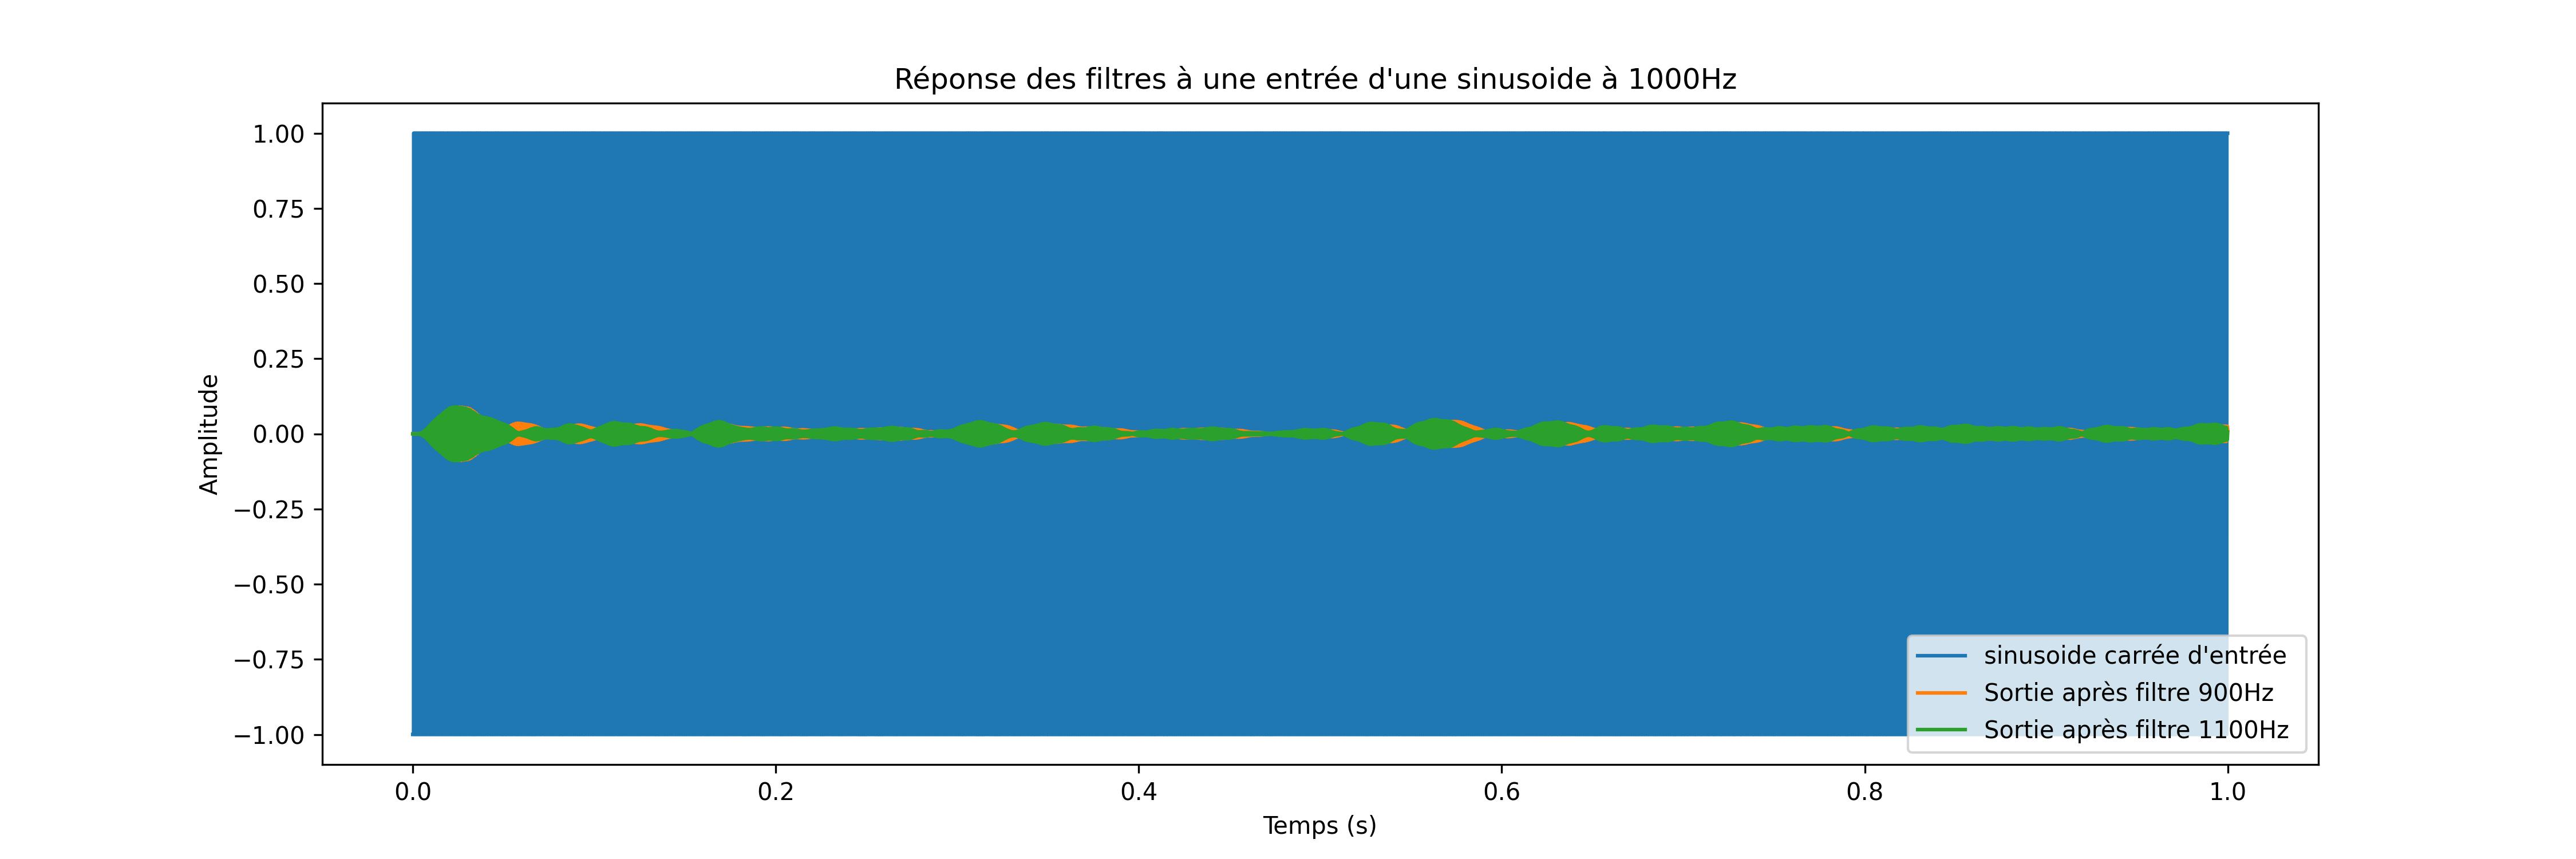
\includegraphics[width=\textwidth]{Pictures/graphique_1000Hz.jpeg}
        \caption{Sinusoïde à 1000Hz}
        \label{fig:image2}
    \end{subfigure}   
    % Troisième image
    \begin{subfigure}[b]{0.75\textwidth}
        \centering
        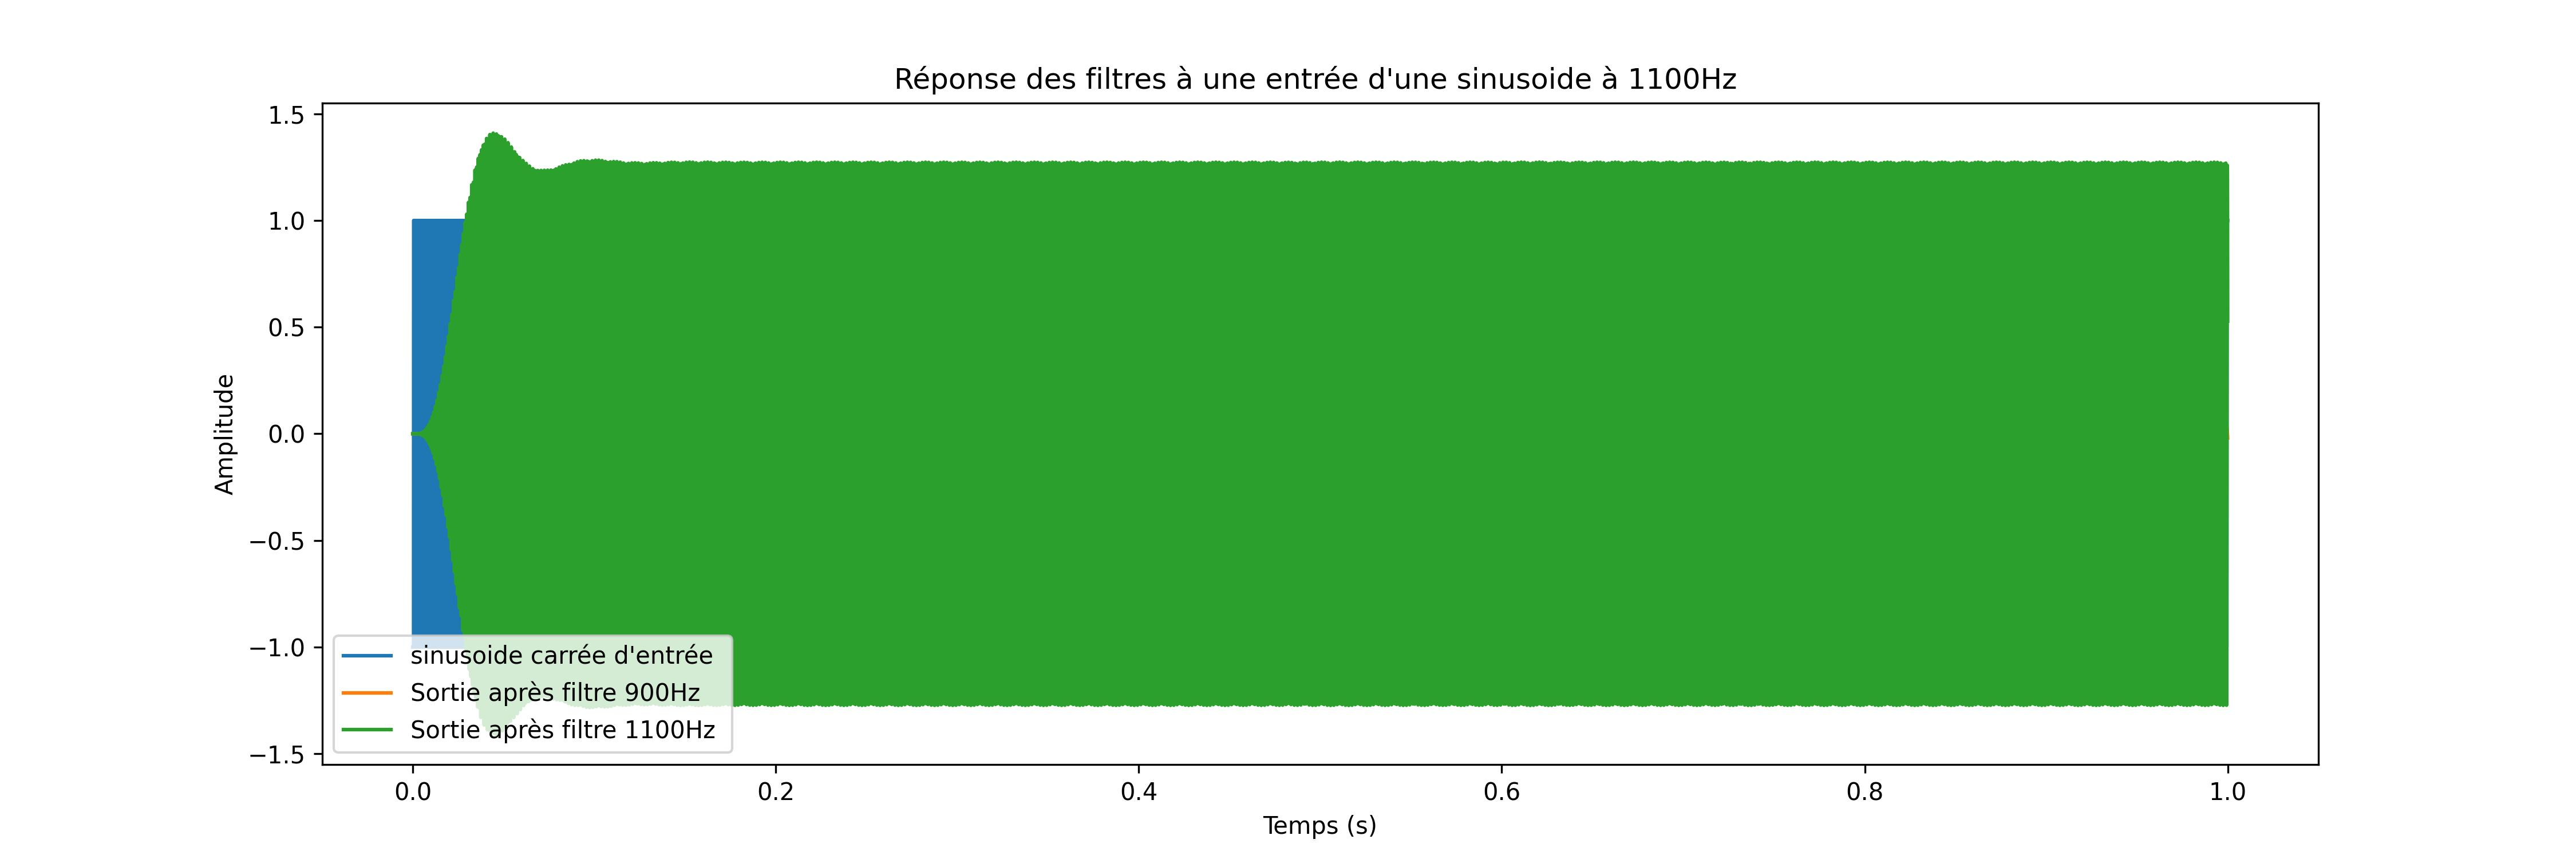
\includegraphics[width=\textwidth]{Pictures/graphique_1100Hz.jpeg}
        \caption{Sinusoïde à 1100Hz}
        \label{fig:image3}
    \end{subfigure}
    \caption{Différentes sorties du filtrage numérique pour des fréquences données}
    \label{fig:subplots}
\end{figure}

Ensuite, les étapes 2 et 3 sont très proches du fait que l'étape 3 est simplement la réimplémentation en C de l'étape 2. Pour ce faire, il a fallu choisir entre précision et temps de calcul. Dans le cadre de ce projet, le processeur étant imposé, le temps de calcul est une contrainte qu'il faut respecter. Différents tests ont été effectués dans le but de connaître nos limites car un grand problème que nous avons rencontré est la gestion d'overflow.

Dans un premier temps, nous avions choisi un décalage de 12 bits (\textit{SCALE\_FACTOR} dans le code), ce qui permettait d'avoir des résultats presque identiques à la simulation en virgule flottante. Cependant, la gestion d'overflow nécessitait une implémentation sur 64 bits pour ne pas perdre de précision. Sachant que la fréquence d'échantillonnage est de 16 kHz, il a fallu s'assurer que le dsPIC puisse effectuer le filtrage dans les deux filtres passe-bandes en moins de $\SI{62,5}{\micro s}$. Cela n'était pas le cas puisque le dsPIC prenait environ $\SI{82}{\micro s}$ sur 64 bits. Le compromis trouvé est d'effectuer les calculs sur 32 bits avec un décalage de 9 bits. C'est également pour réduire le temps de calcul que la fréquence du dsPic a été augmentée à $40MHz$. Les allures des sorties obtenues dans ce cas sont les suivante :

\begin{figure}[H]
    \centering
    % Première image
    \begin{subfigure}[b]{0.7\textwidth}
        \centering
        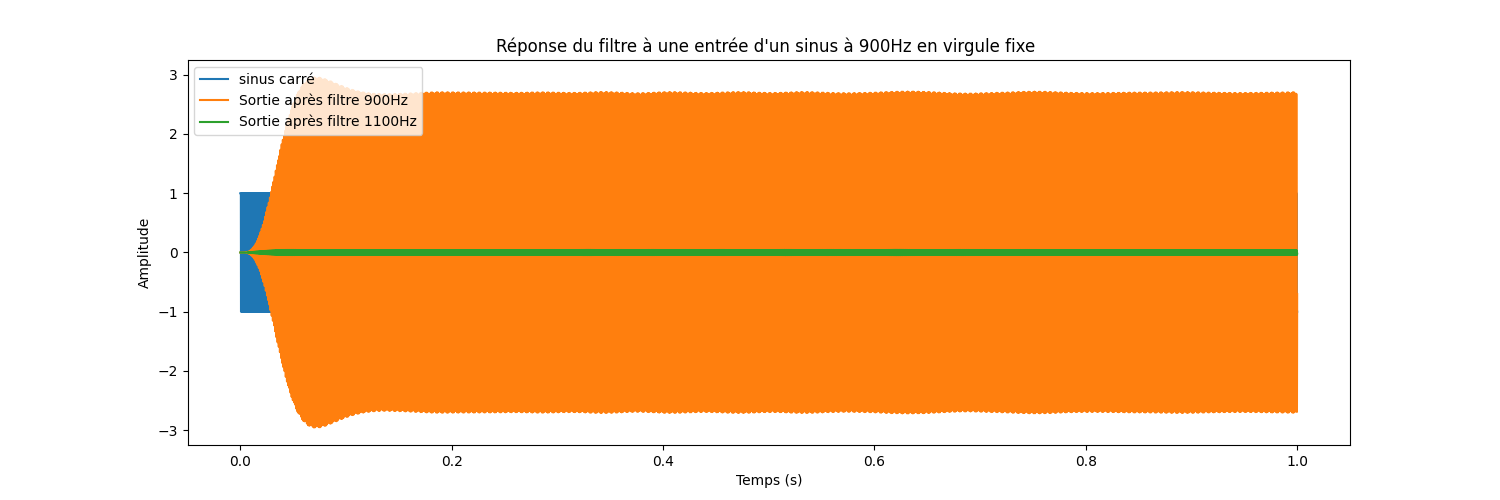
\includegraphics[width=\textwidth]{Pictures/virgule_fixe_900.png}
        \caption{Sortie de la sinusoide à 900Hz}
        \label{fig:image1}
    \end{subfigure}
    % Deuxième image
    \begin{subfigure}[b]{0.7\textwidth}
        \centering
        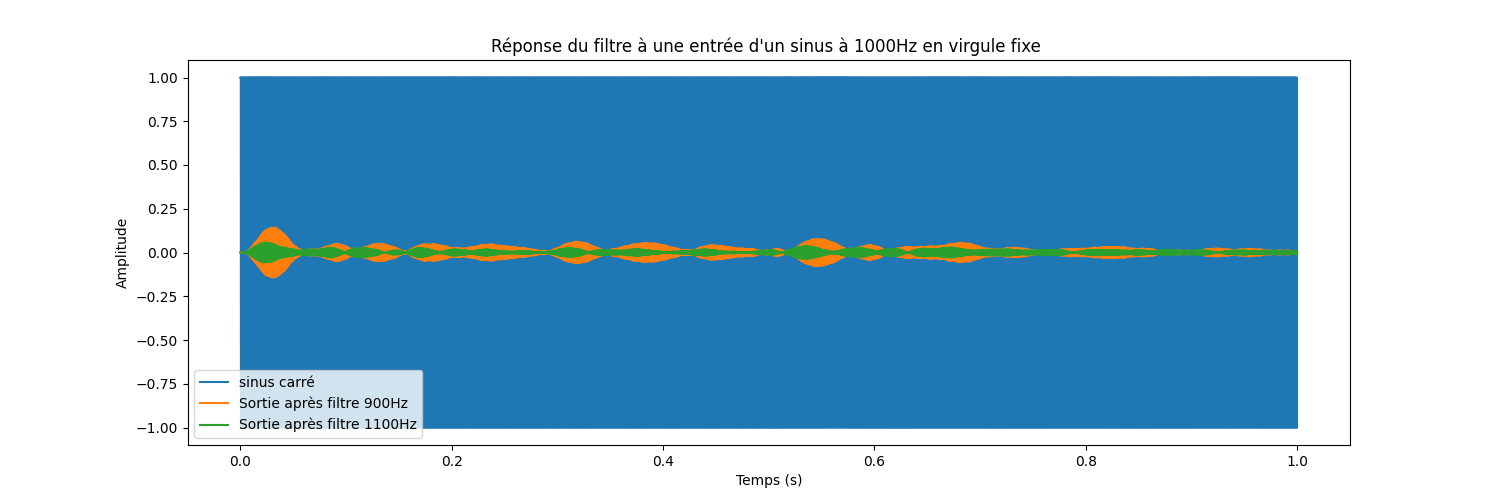
\includegraphics[width=\textwidth]{Pictures/virgule_fixe1000.png}
        \caption{Sinusoïde à 1000Hz}
        \label{fig:image2}
    \end{subfigure}   
    % Troisième image
    \begin{subfigure}[b]{0.7\textwidth}
        \centering
        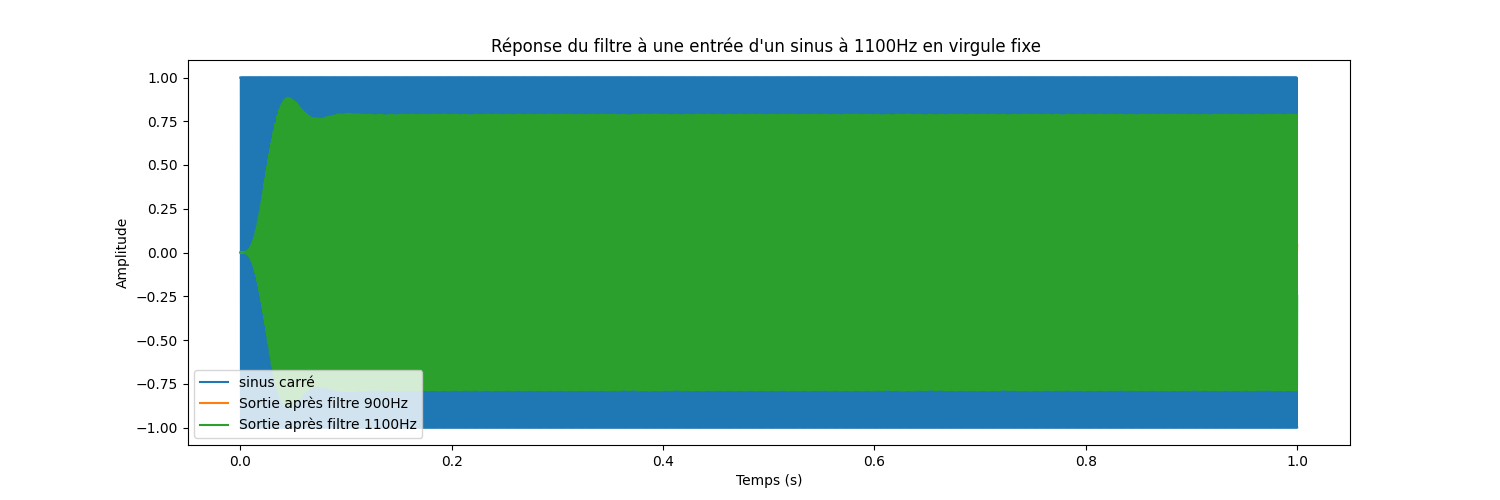
\includegraphics[width=\textwidth]{Pictures/test_virgule_fixe_1100.png}
        \caption{Sinusoïde à 1100Hz}
        \label{fig:image3}
    \end{subfigure}
    \caption{Différentes sorties du filtrage numérique pour des fréquences données}
    \label{fig:subplots}
\end{figure}
Il est possible de voir que le filtre à 900 Hz tend vers une amplitude de $\pm3$ alors que celui à 1100 Hz tend vers $\pm 0.75$, ce qui est tout de même assez différent de notre cas en virgule flottante. Ces différences s'expliquent par la perte de précision du modèle en virgule fixe établi sous les contraintes expliquées ci-dessus. Les valeurs maximales de sortie de ces filtres seront importantes pour le détecteur d'amplitude qui sera expliqué par après.
\subsection{Test Réel}
Une fois le filtre numérique validé. Différents essais ont été réalisé avec le signal reçu par l'ADC comme entrée. Il a fallu s'assurer que le processus prenne moins de $62.5 \mu s$ et que le signal soit également correctement filtré. Pour ce faire, un son aux différentes fréquences a été émis. Les résultats de ces tests sont disponibles sur les figures \ref{fig:filtre1100test}, \ref{fig:filtre900test} et \ref{fig:timefiltre}. Il est important de noter que pour ces résultats, la fenêtre glissante (\ref{fenetre_glissante}) a déjà été implémentée.

\begin{figure}[H]
    \centering
    \begin{subfigure}[b]{\textwidth}
        \centering
        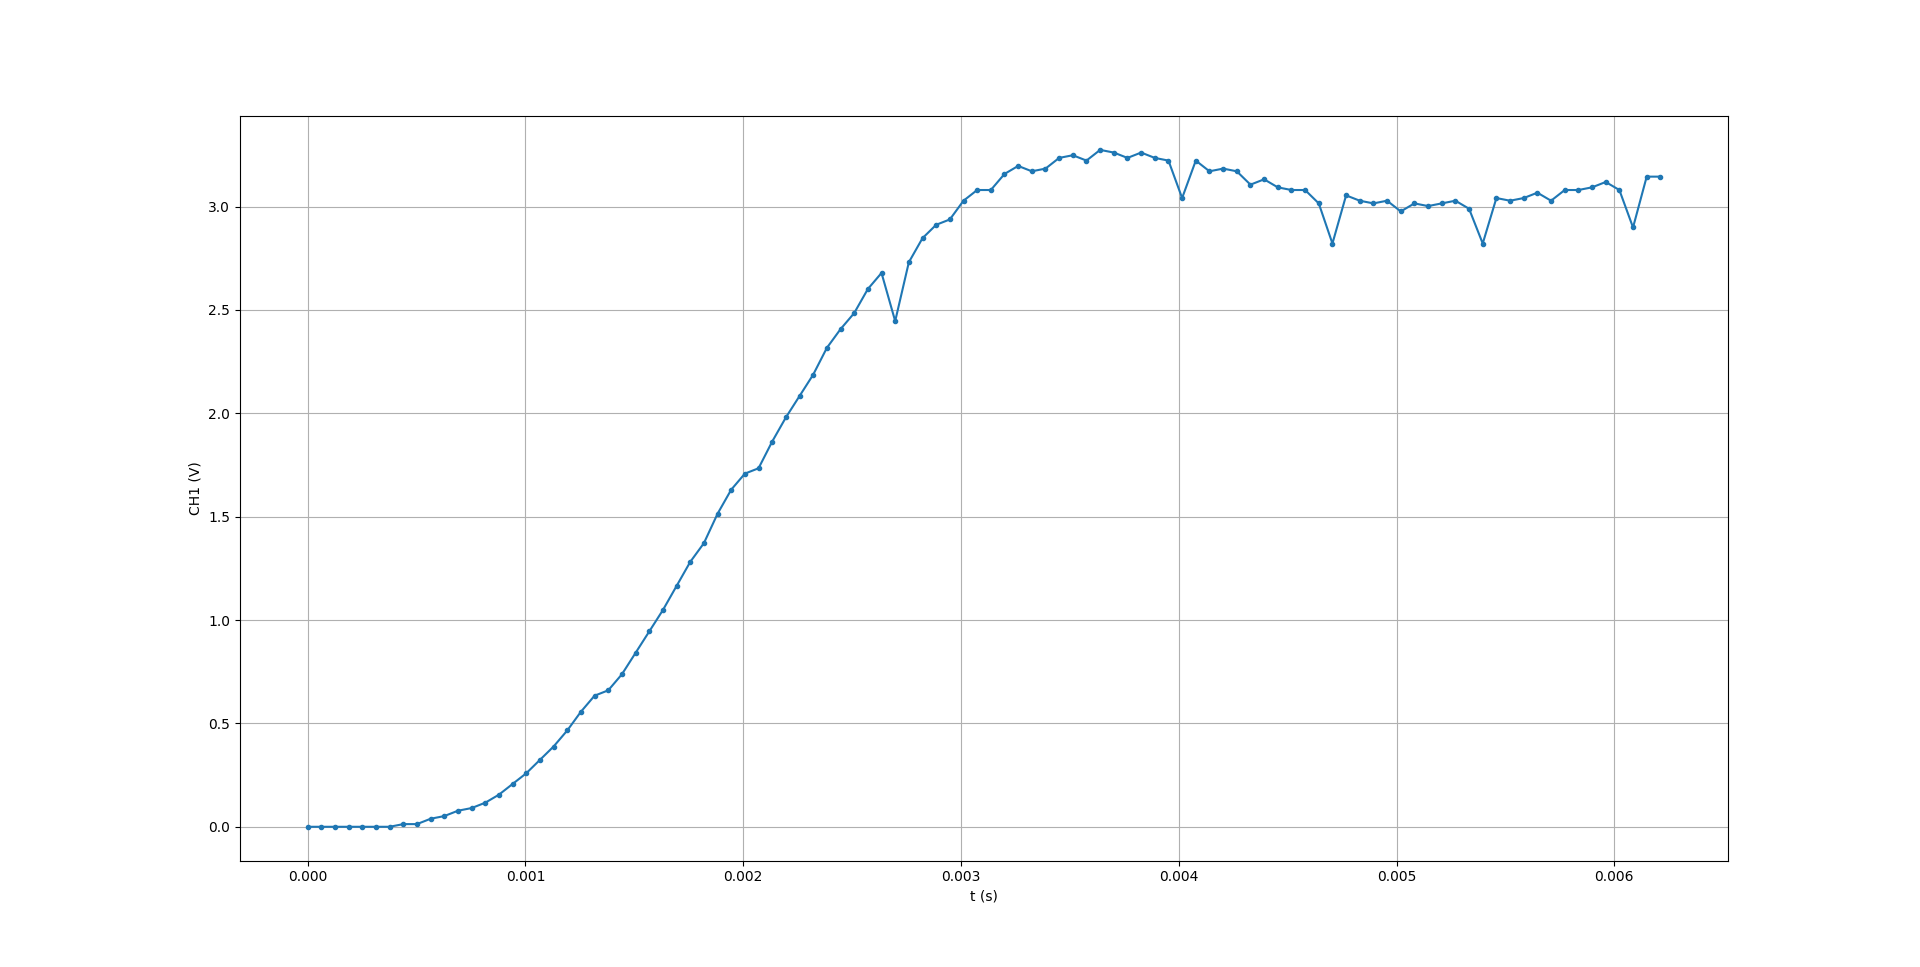
\includegraphics[width=\textwidth]{Pictures/fil900-900.png}
        \caption{Résultat oscilloscope du filtre de 900 Hz pour une entrée de 900 Hz}
        \label{fig:900-900}
    \end{subfigure}
    \begin{subfigure}[b]{\textwidth}
        \centering
        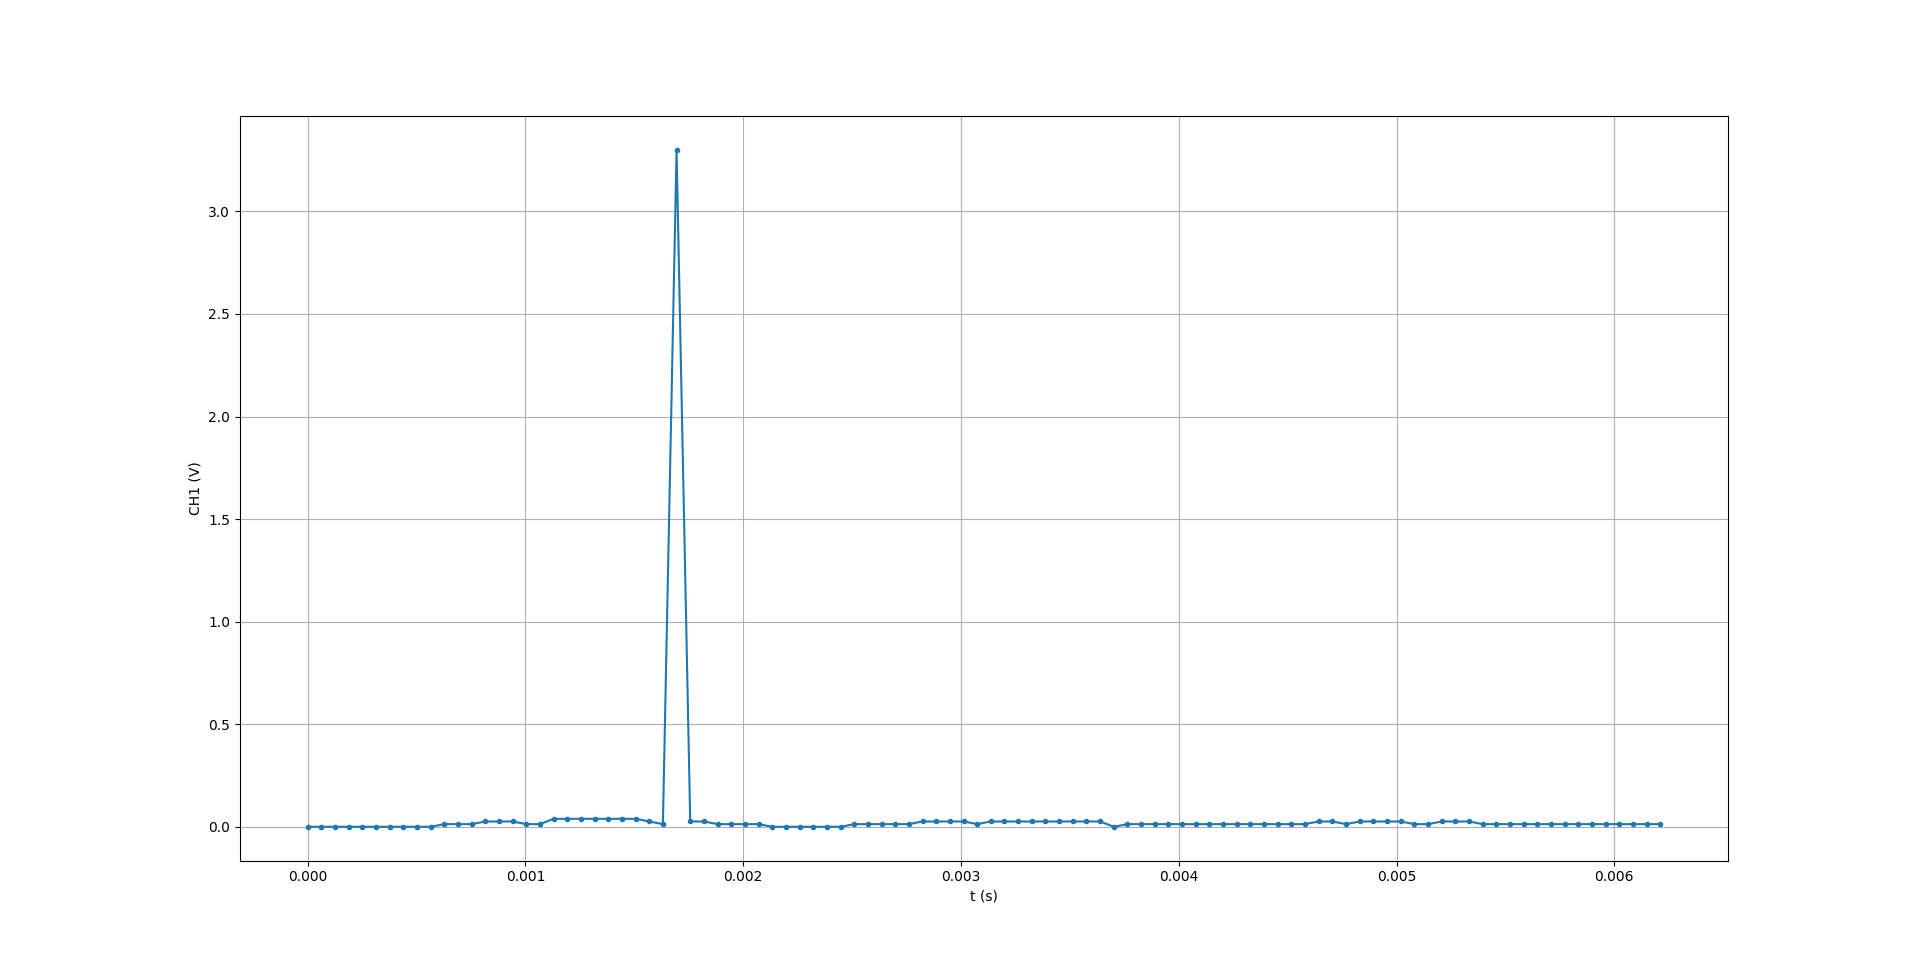
\includegraphics[width=\textwidth]{Pictures/fil900-1100.png}
        \caption{Résultat oscilloscope du filtre de 900 Hz pour une entrée de 1100 Hz}
        \label{fig:900-1100}
    \end{subfigure}
    \caption{Ensemble des résultats pour le filtre 900 Hz}
    \label{fig:filtre900test}
\end{figure}

\begin{figure}[H]
    \centering
\begin{subfigure}[b]{\textwidth}
    \centering
    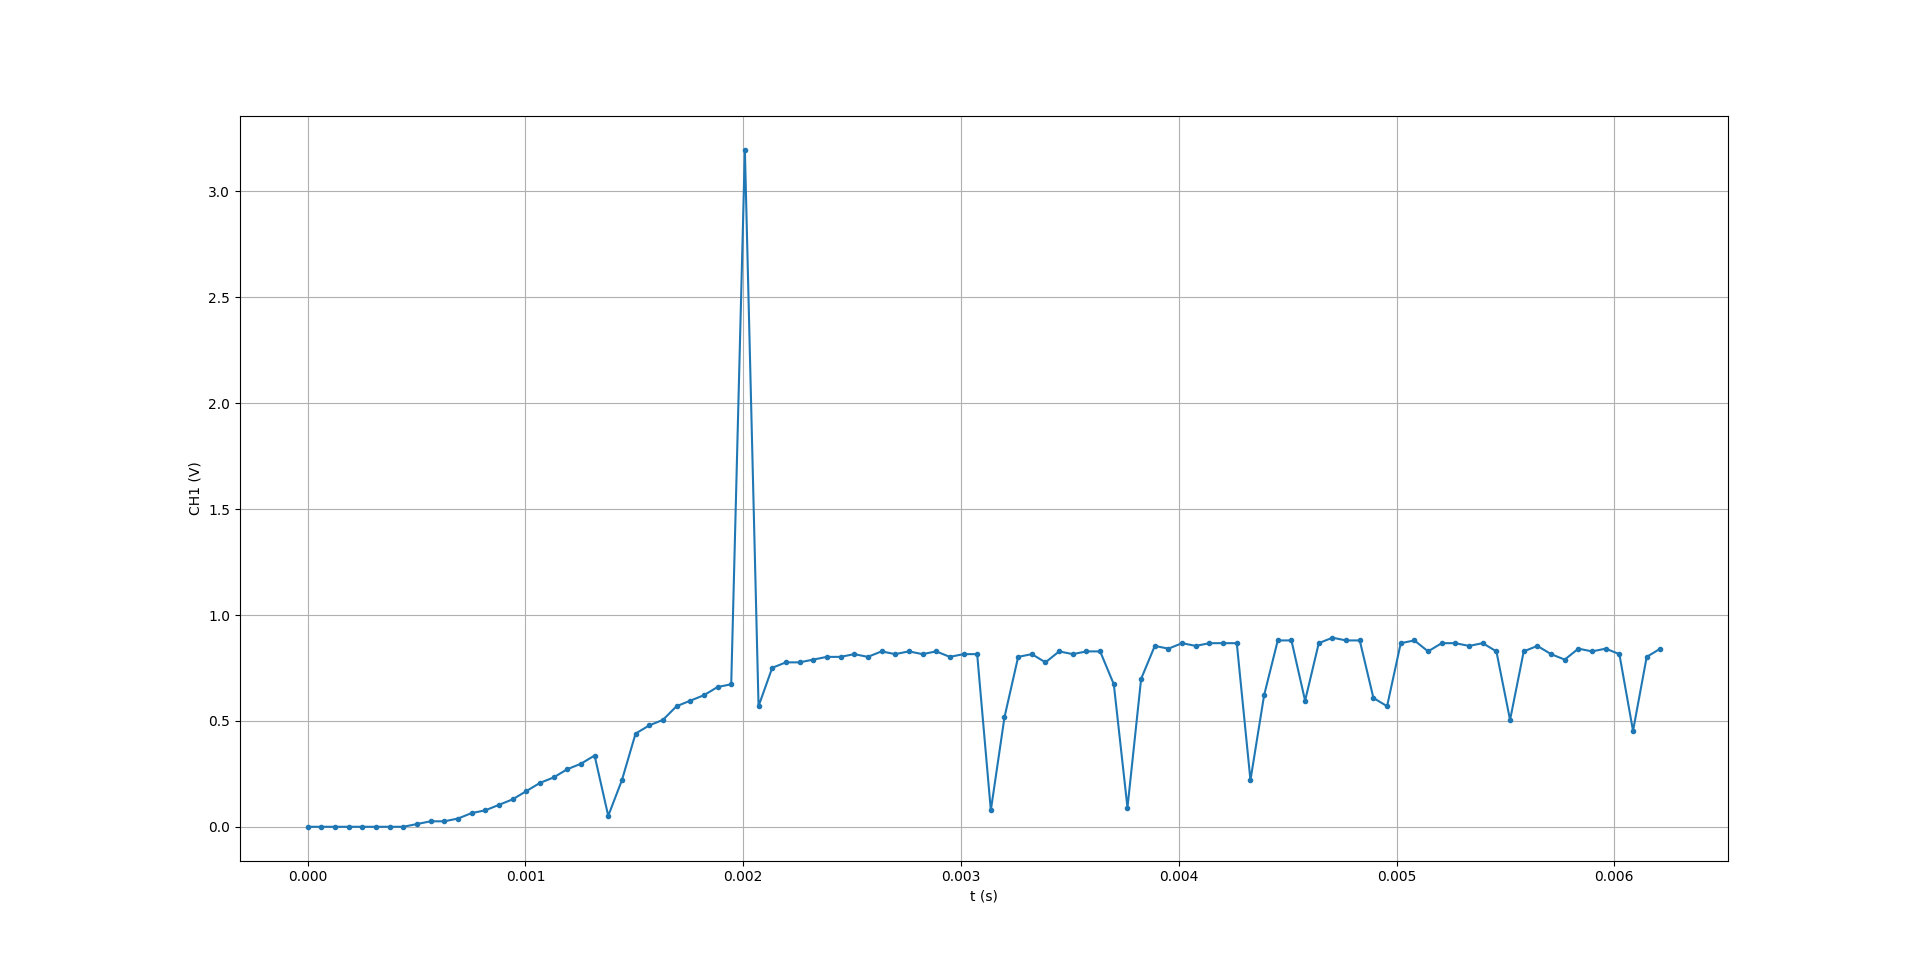
\includegraphics[width=\textwidth]{Pictures/fil1100-1100.png}
    \caption{Résultat oscilloscope du filtre de 1100 Hz pour une entrée de 1100 Hz}
    \label{fig:1100-1100}
\end{subfigure}

\begin{subfigure}[b]{\textwidth}
    \centering
    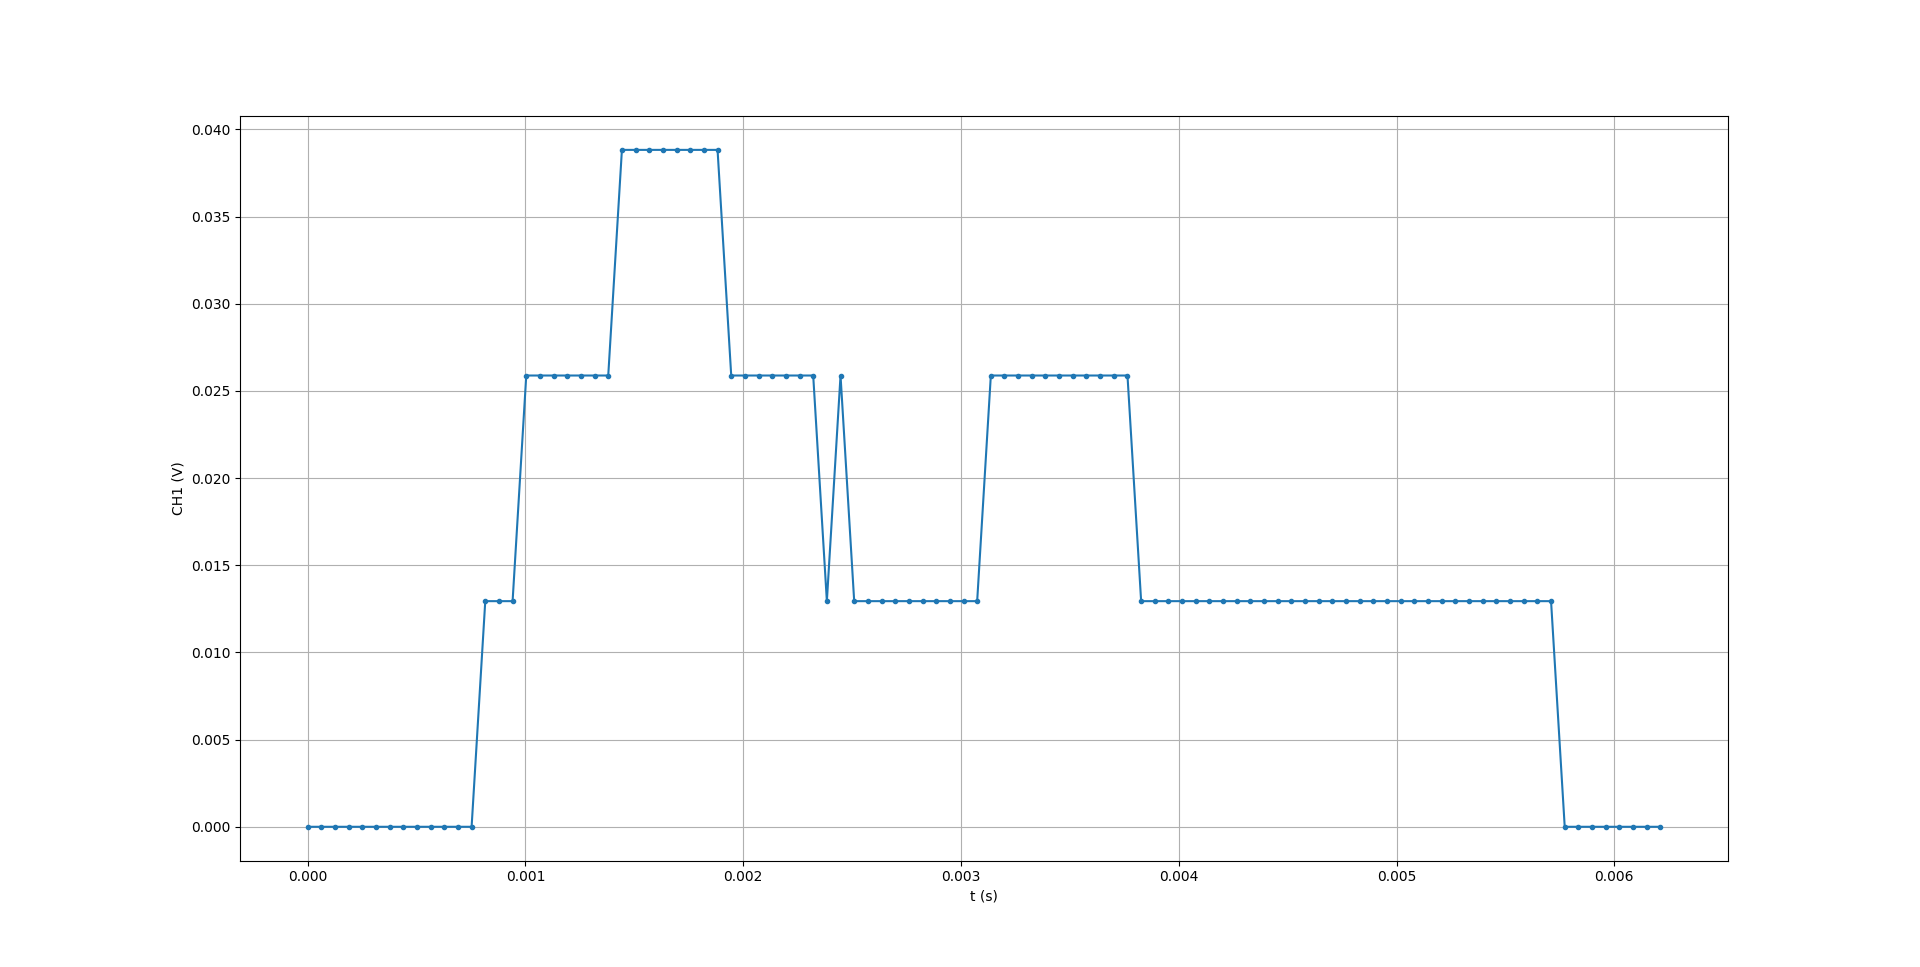
\includegraphics[width=\textwidth]{Pictures/fil1100-900.png}
    \caption{Résultat oscilloscope du filtre de 1100 Hz pour une entrée de 900 Hz}
    \label{fig:1100-900}
\end{subfigure}

\caption{Ensemble des résultats pour le filtre 1100 Hz}
    \label{fig:filtre1100test}
\end{figure}

\begin{figure}[H]
    \centering
    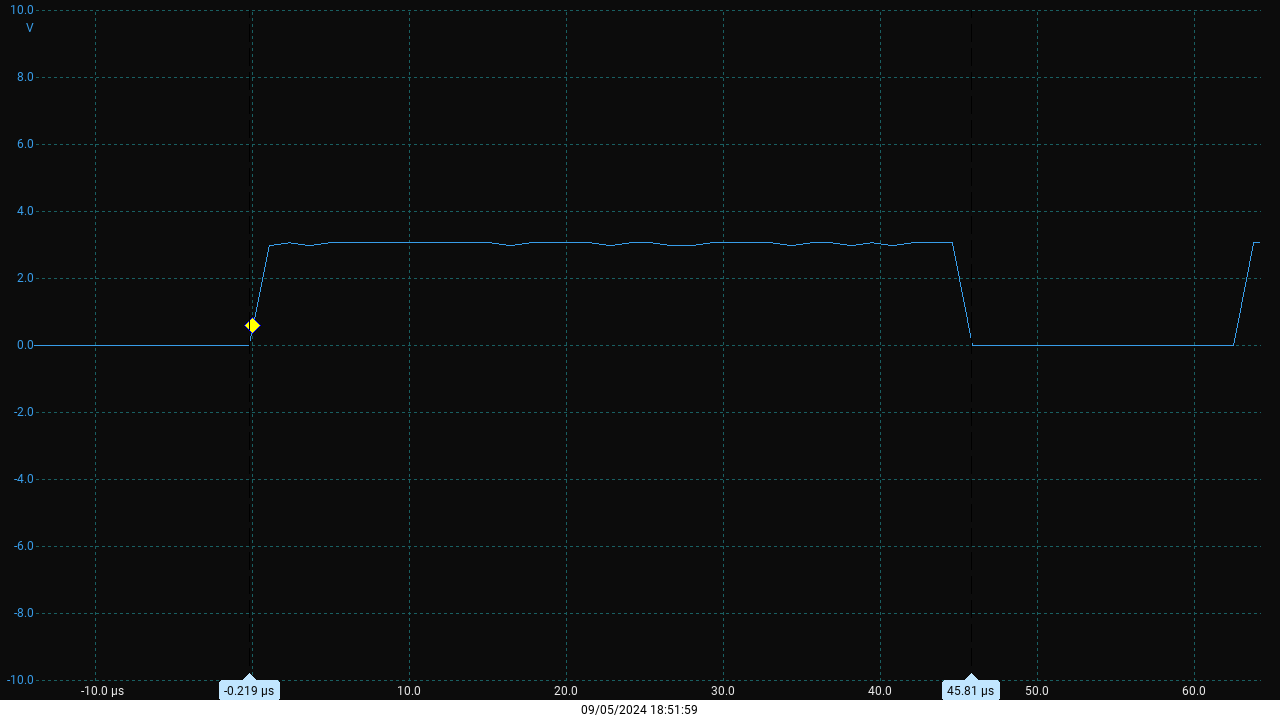
\includegraphics[scale=0.35]{Pictures/TimeFIlter.png}
    \caption{Temps de calcul du microcontrôleur pour exécuter les filtres numériques}
    \label{fig:timefiltre}
\end{figure}

